\documentclass[journal]{IEEEtran}
\IEEEoverridecommandlockouts
% Shared by bpp_v3_conf.tex and bpp_v3_journal.tex
\usepackage{amsmath,amssymb}
\usepackage{graphicx}
\usepackage{booktabs}
\usepackage{xurl}
\usepackage{cite}
\usepackage{xspace}
\usepackage[table]{xcolor}
\graphicspath{{figures/}}

% System name in one place: change here to rename everywhere.
\newcommand{\sysname}{BioPathNet++\xspace}

% Every number below is generated by `python -m bpp.analyze` from the run logs;
% never type a result by hand in the papers.
\newcommand{\MainValidMrr}{0.394}
\newcommand{\MainValidMrrSd}{0.003}
\newcommand{\MainValidHitsOne}{0.353}
\newcommand{\MainValidHitsOneSd}{0.008}
\newcommand{\MainValidHitsTen}{0.456}
\newcommand{\MainValidHitsTenSd}{0.018}
\newcommand{\MainValidHitsHundred}{0.669}
\newcommand{\MainValidHitsHundredSd}{0.021}
\newcommand{\MainValidAuroc}{0.938}
\newcommand{\MainValidAurocSd}{0.001}
\newcommand{\MainValidAuprc}{0.424}
\newcommand{\MainValidAuprcSd}{0.005}
\newcommand{\MainValidAurocHard}{0.799}
\newcommand{\MainValidAurocHardSd}{0.010}
\newcommand{\MainValidAurocDeg}{0.886}
\newcommand{\MainValidAurocDegSd}{0.010}
\newcommand{\MainValidAnyTen}{56}
\newcommand{\MainTargetsMrr}{0.475}
\newcommand{\MainTargetsMrrSd}{0.017}
\newcommand{\MainTargetsHitsOne}{0.396}
\newcommand{\MainTargetsHitsOneSd}{0.038}
\newcommand{\MainTargetsHitsTen}{0.648}
\newcommand{\MainTargetsHitsTenSd}{0.033}
\newcommand{\MainTargetsHitsHundred}{0.716}
\newcommand{\MainTargetsHitsHundredSd}{0.016}
\newcommand{\MainTargetsAuroc}{0.982}
\newcommand{\MainTargetsAurocSd}{0.008}
\newcommand{\MainTargetsAuprc}{0.594}
\newcommand{\MainTargetsAuprcSd}{0.010}
\newcommand{\MainTargetsAurocHard}{0.892}
\newcommand{\MainTargetsAurocHardSd}{0.020}
\newcommand{\MainTargetsAurocDeg}{0.954}
\newcommand{\MainTargetsAurocDegSd}{0.031}
\newcommand{\MainTargetsAnyTen}{83}
\newcommand{\MainSeeds}{3}
\newcommand{\PathsValidMrr}{0.405}
\newcommand{\PathsValidMrrSd}{0.013}
\newcommand{\PathsValidHitsOne}{0.363}
\newcommand{\PathsValidHitsOneSd}{0.019}
\newcommand{\PathsValidHitsTen}{0.479}
\newcommand{\PathsValidHitsTenSd}{0.025}
\newcommand{\PathsValidHitsHundred}{0.663}
\newcommand{\PathsValidHitsHundredSd}{0.018}
\newcommand{\PathsValidAuroc}{0.946}
\newcommand{\PathsValidAurocSd}{0.004}
\newcommand{\PathsValidAuprc}{0.443}
\newcommand{\PathsValidAuprcSd}{0.010}
\newcommand{\PathsValidAurocHard}{0.829}
\newcommand{\PathsValidAurocHardSd}{0.011}
\newcommand{\PathsValidAurocDeg}{0.888}
\newcommand{\PathsValidAurocDegSd}{0.009}
\newcommand{\PathsValidAnyTen}{59}
\newcommand{\PathsTargetsMrr}{0.463}
\newcommand{\PathsTargetsMrrSd}{0.087}
\newcommand{\PathsTargetsHitsOne}{0.375}
\newcommand{\PathsTargetsHitsOneSd}{0.134}
\newcommand{\PathsTargetsHitsTen}{0.657}
\newcommand{\PathsTargetsHitsTenSd}{0.025}
\newcommand{\PathsTargetsHitsHundred}{0.738}
\newcommand{\PathsTargetsHitsHundredSd}{0.023}
\newcommand{\PathsTargetsAuroc}{0.986}
\newcommand{\PathsTargetsAurocSd}{0.004}
\newcommand{\PathsTargetsAuprc}{0.577}
\newcommand{\PathsTargetsAuprcSd}{0.054}
\newcommand{\PathsTargetsAurocHard}{0.907}
\newcommand{\PathsTargetsAurocHardSd}{0.007}
\newcommand{\PathsTargetsAurocDeg}{0.968}
\newcommand{\PathsTargetsAurocDegSd}{0.015}
\newcommand{\PathsTargetsAnyTen}{83}
\newcommand{\PathsSeeds}{3}
\newcommand{\PriorValidMrr}{0.303}
\newcommand{\PriorValidMrrSd}{--}
\newcommand{\PriorValidHitsOne}{0.265}
\newcommand{\PriorValidHitsOneSd}{--}
\newcommand{\PriorValidHitsTen}{0.353}
\newcommand{\PriorValidHitsTenSd}{--}
\newcommand{\PriorValidHitsHundred}{0.536}
\newcommand{\PriorValidHitsHundredSd}{--}
\newcommand{\PriorValidAuroc}{0.884}
\newcommand{\PriorValidAurocSd}{--}
\newcommand{\PriorValidAuprc}{0.334}
\newcommand{\PriorValidAuprcSd}{--}
\newcommand{\PriorValidAurocHard}{0.707}
\newcommand{\PriorValidAurocHardSd}{--}
\newcommand{\PriorValidAurocDeg}{0.843}
\newcommand{\PriorValidAurocDegSd}{--}
\newcommand{\PriorValidAnyTen}{46}
\newcommand{\PriorTargetsMrr}{0.322}
\newcommand{\PriorTargetsMrrSd}{--}
\newcommand{\PriorTargetsHitsOne}{0.243}
\newcommand{\PriorTargetsHitsOneSd}{--}
\newcommand{\PriorTargetsHitsTen}{0.483}
\newcommand{\PriorTargetsHitsTenSd}{--}
\newcommand{\PriorTargetsHitsHundred}{0.718}
\newcommand{\PriorTargetsHitsHundredSd}{--}
\newcommand{\PriorTargetsAuroc}{0.955}
\newcommand{\PriorTargetsAurocSd}{--}
\newcommand{\PriorTargetsAuprc}{0.443}
\newcommand{\PriorTargetsAuprcSd}{--}
\newcommand{\PriorTargetsAurocHard}{0.782}
\newcommand{\PriorTargetsAurocHardSd}{--}
\newcommand{\PriorTargetsAurocDeg}{0.909}
\newcommand{\PriorTargetsAurocDegSd}{--}
\newcommand{\PriorTargetsAnyTen}{83}
\newcommand{\PriorSeeds}{1}
\newcommand{\NoautoValidMrr}{0.454}
\newcommand{\NoautoValidMrrSd}{--}
\newcommand{\NoautoValidHitsOne}{0.400}
\newcommand{\NoautoValidHitsOneSd}{--}
\newcommand{\NoautoValidHitsTen}{0.557}
\newcommand{\NoautoValidHitsTenSd}{--}
\newcommand{\NoautoValidHitsHundred}{0.719}
\newcommand{\NoautoValidHitsHundredSd}{--}
\newcommand{\NoautoValidAuroc}{0.946}
\newcommand{\NoautoValidAurocSd}{--}
\newcommand{\NoautoValidAuprc}{0.489}
\newcommand{\NoautoValidAuprcSd}{--}
\newcommand{\NoautoValidAurocHard}{0.838}
\newcommand{\NoautoValidAurocHardSd}{--}
\newcommand{\NoautoValidAurocDeg}{0.891}
\newcommand{\NoautoValidAurocDegSd}{--}
\newcommand{\NoautoValidAnyTen}{70}
\newcommand{\NoautoTargetsMrr}{0.473}
\newcommand{\NoautoTargetsMrrSd}{--}
\newcommand{\NoautoTargetsHitsOne}{0.404}
\newcommand{\NoautoTargetsHitsOneSd}{--}
\newcommand{\NoautoTargetsHitsTen}{0.628}
\newcommand{\NoautoTargetsHitsTenSd}{--}
\newcommand{\NoautoTargetsHitsHundred}{0.711}
\newcommand{\NoautoTargetsHitsHundredSd}{--}
\newcommand{\NoautoTargetsAuroc}{0.975}
\newcommand{\NoautoTargetsAurocSd}{--}
\newcommand{\NoautoTargetsAuprc}{0.576}
\newcommand{\NoautoTargetsAuprcSd}{--}
\newcommand{\NoautoTargetsAurocHard}{0.899}
\newcommand{\NoautoTargetsAurocHardSd}{--}
\newcommand{\NoautoTargetsAurocDeg}{0.914}
\newcommand{\NoautoTargetsAurocDegSd}{--}
\newcommand{\NoautoTargetsAnyTen}{83}
\newcommand{\NoautoAreaMrr}{0.485}
\newcommand{\NoautoAreaMrrSd}{--}
\newcommand{\NoautoAreaHitsOne}{0.406}
\newcommand{\NoautoAreaHitsOneSd}{--}
\newcommand{\NoautoAreaHitsTen}{0.608}
\newcommand{\NoautoAreaHitsTenSd}{--}
\newcommand{\NoautoAreaHitsHundred}{0.717}
\newcommand{\NoautoAreaHitsHundredSd}{--}
\newcommand{\NoautoAreaAuroc}{0.947}
\newcommand{\NoautoAreaAurocSd}{--}
\newcommand{\NoautoAreaAuprc}{0.528}
\newcommand{\NoautoAreaAuprcSd}{--}
\newcommand{\NoautoAreaAurocHard}{0.816}
\newcommand{\NoautoAreaAurocHardSd}{--}
\newcommand{\NoautoAreaAurocDeg}{0.913}
\newcommand{\NoautoAreaAurocDegSd}{--}
\newcommand{\NoautoAreaAnyTen}{76}
\newcommand{\NoautoSeeds}{1}
\newcommand{\KnnValidMrr}{0.281}
\newcommand{\KnnValidHitsTen}{0.350}
\newcommand{\KnnValidAuroc}{0.860}
\newcommand{\KnnValidAurocHard}{0.661}
\newcommand{\KnnValidAnyTen}{44}
\newcommand{\KnnTargetsMrr}{0.296}
\newcommand{\KnnTargetsHitsTen}{0.424}
\newcommand{\KnnTargetsAuroc}{0.962}
\newcommand{\KnnTargetsAurocHard}{0.778}
\newcommand{\KnnTargetsAnyTen}{67}
\newcommand{\PopValidMrr}{0.046}
\newcommand{\PopValidHitsTen}{0.049}
\newcommand{\PopValidAuroc}{0.830}
\newcommand{\PopValidAurocHard}{0.476}
\newcommand{\PopValidAnyTen}{15}
\newcommand{\PopTargetsMrr}{0.099}
\newcommand{\PopTargetsHitsTen}{0.148}
\newcommand{\PopTargetsAuroc}{0.905}
\newcommand{\PopTargetsAurocHard}{0.460}
\newcommand{\PopTargetsAnyTen}{50}
\newcommand{\RandValidMrr}{0.001}
\newcommand{\RandValidHitsTen}{0.002}
\newcommand{\RandValidAuroc}{0.471}
\newcommand{\RandValidAurocHard}{0.488}
\newcommand{\RandValidAnyTen}{1}
\newcommand{\RandTargetsMrr}{0.001}
\newcommand{\RandTargetsHitsTen}{0.000}
\newcommand{\RandTargetsAuroc}{0.476}
\newcommand{\RandTargetsAurocHard}{0.488}
\newcommand{\RandTargetsAnyTen}{0}
\newcommand{\DegValidMrr}{0.004}
\newcommand{\DegValidHitsTen}{0.003}
\newcommand{\DegValidAuroc}{0.783}
\newcommand{\DegValidAurocHard}{0.421}
\newcommand{\DegValidAnyTen}{1}
\newcommand{\DegTargetsMrr}{0.003}
\newcommand{\DegTargetsHitsTen}{0.000}
\newcommand{\DegTargetsAuroc}{0.732}
\newcommand{\DegTargetsAurocHard}{0.404}
\newcommand{\DegTargetsAnyTen}{0}
\newcommand{\NoautoKnnValidMrr}{0.347}
\newcommand{\NoautoKnnValidHitsTen}{0.407}
\newcommand{\NoautoKnnValidAuroc}{0.890}
\newcommand{\NoautoKnnValidAurocHard}{0.748}
\newcommand{\NoautoKnnValidAnyTen}{53}
\newcommand{\NoautoKnnTargetsMrr}{0.273}
\newcommand{\NoautoKnnTargetsHitsTen}{0.594}
\newcommand{\NoautoKnnTargetsAuroc}{0.857}
\newcommand{\NoautoKnnTargetsAurocHard}{0.790}
\newcommand{\NoautoKnnTargetsAnyTen}{83}
\newcommand{\NoautoKnnAreaMrr}{0.311}
\newcommand{\NoautoKnnAreaHitsTen}{0.469}
\newcommand{\NoautoKnnAreaAuroc}{0.832}
\newcommand{\NoautoKnnAreaAurocHard}{0.712}
\newcommand{\NoautoKnnAreaAnyTen}{57}
\newcommand{\NoautoPopValidMrr}{0.054}
\newcommand{\NoautoPopValidHitsTen}{0.054}
\newcommand{\NoautoPopValidAuroc}{0.871}
\newcommand{\NoautoPopValidAurocHard}{0.639}
\newcommand{\NoautoPopValidAnyTen}{12}
\newcommand{\NoautoPopTargetsMrr}{0.093}
\newcommand{\NoautoPopTargetsHitsTen}{0.148}
\newcommand{\NoautoPopTargetsAuroc}{0.799}
\newcommand{\NoautoPopTargetsAurocHard}{0.519}
\newcommand{\NoautoPopTargetsAnyTen}{50}
\newcommand{\NoautoPopAreaMrr}{0.260}
\newcommand{\NoautoPopAreaHitsTen}{0.346}
\newcommand{\NoautoPopAreaAuroc}{0.808}
\newcommand{\NoautoPopAreaAurocHard}{0.604}
\newcommand{\NoautoPopAreaAnyTen}{48}
\newcommand{\NoautoRandValidMrr}{0.001}
\newcommand{\NoautoRandValidHitsTen}{0.005}
\newcommand{\NoautoRandValidAuroc}{0.428}
\newcommand{\NoautoRandValidAurocHard}{0.443}
\newcommand{\NoautoRandValidAnyTen}{2}
\newcommand{\NoautoRandTargetsMrr}{0.001}
\newcommand{\NoautoRandTargetsHitsTen}{0.000}
\newcommand{\NoautoRandTargetsAuroc}{0.476}
\newcommand{\NoautoRandTargetsAurocHard}{0.488}
\newcommand{\NoautoRandTargetsAnyTen}{0}
\newcommand{\NoautoRandAreaMrr}{0.000}
\newcommand{\NoautoRandAreaHitsTen}{0.000}
\newcommand{\NoautoRandAreaAuroc}{0.419}
\newcommand{\NoautoRandAreaAurocHard}{0.436}
\newcommand{\NoautoRandAreaAnyTen}{0}
\newcommand{\NoautoDegValidMrr}{0.003}
\newcommand{\NoautoDegValidHitsTen}{0.001}
\newcommand{\NoautoDegValidAuroc}{0.778}
\newcommand{\NoautoDegValidAurocHard}{0.435}
\newcommand{\NoautoDegValidAnyTen}{2}
\newcommand{\NoautoDegTargetsMrr}{0.003}
\newcommand{\NoautoDegTargetsHitsTen}{0.000}
\newcommand{\NoautoDegTargetsAuroc}{0.732}
\newcommand{\NoautoDegTargetsAurocHard}{0.404}
\newcommand{\NoautoDegTargetsAnyTen}{0}
\newcommand{\NoautoDegAreaMrr}{0.003}
\newcommand{\NoautoDegAreaHitsTen}{0.000}
\newcommand{\NoautoDegAreaAuroc}{0.820}
\newcommand{\NoautoDegAreaAurocHard}{0.443}
\newcommand{\NoautoDegAreaAnyTen}{0}
\newcommand{\DiffMainKnnValid}{+0.113}
\newcommand{\PbootMainKnnValid}{$<$0.001}
\newcommand{\PwilMainKnnValid}{$<$0.001}
\newcommand{\DiffLoMainKnnValid}{+0.056}
\newcommand{\DiffHiMainKnnValid}{+0.179}
\newcommand{\WinsMainKnnValid}{43}
\newcommand{\TiesMainKnnValid}{13}
\newcommand{\LossesMainKnnValid}{12}
\newcommand{\DiffMainKnnTargets}{+0.179}
\newcommand{\PbootMainKnnTargets}{$=$0.043}
\newcommand{\PwilMainKnnTargets}{$=$0.188}
\newcommand{\DiffLoMainKnnTargets}{-0.027}
\newcommand{\DiffHiMainKnnTargets}{+0.370}
\newcommand{\WinsMainKnnTargets}{4}
\newcommand{\TiesMainKnnTargets}{1}
\newcommand{\LossesMainKnnTargets}{1}
\newcommand{\DiffMainPathsValid}{-0.010}
\newcommand{\PbootMainPathsValid}{$=$0.752}
\newcommand{\PwilMainPathsValid}{$=$0.148}
\newcommand{\DiffLoMainPathsValid}{-0.043}
\newcommand{\DiffHiMainPathsValid}{+0.021}
\newcommand{\WinsMainPathsValid}{19}
\newcommand{\TiesMainPathsValid}{14}
\newcommand{\LossesMainPathsValid}{35}
\newcommand{\DiffMainPathsTargets}{+0.011}
\newcommand{\PbootMainPathsTargets}{$=$0.359}
\newcommand{\PwilMainPathsTargets}{$=$0.625}
\newcommand{\DiffLoMainPathsTargets}{-0.105}
\newcommand{\DiffHiMainPathsTargets}{+0.129}
\newcommand{\WinsMainPathsTargets}{3}
\newcommand{\TiesMainPathsTargets}{1}
\newcommand{\LossesMainPathsTargets}{2}
\newcommand{\DiffMainNoautoTargets}{+0.002}
\newcommand{\PbootMainNoautoTargets}{$=$0.435}
\newcommand{\PwilMainNoautoTargets}{$=$0.625}
\newcommand{\DiffLoMainNoautoTargets}{-0.090}
\newcommand{\DiffHiMainNoautoTargets}{+0.078}
\newcommand{\WinsMainNoautoTargets}{4}
\newcommand{\TiesMainNoautoTargets}{1}
\newcommand{\LossesMainNoautoTargets}{1}
\newcommand{\DiffNoautoKnnArea}{+0.174}
\newcommand{\PbootNoautoKnnArea}{$=$0.005}
\newcommand{\PwilNoautoKnnArea}{$=$0.085}
\newcommand{\DiffLoNoautoKnnArea}{+0.033}
\newcommand{\DiffHiNoautoKnnArea}{+0.326}
\newcommand{\WinsNoautoKnnArea}{12}
\newcommand{\TiesNoautoKnnArea}{3}
\newcommand{\LossesNoautoKnnArea}{6}
\newcommand{\DiffPathsKnnValid}{+0.124}
\newcommand{\PbootPathsKnnValid}{$<$0.001}
\newcommand{\PwilPathsKnnValid}{$<$0.001}
\newcommand{\DiffLoPathsKnnValid}{+0.057}
\newcommand{\DiffHiPathsKnnValid}{+0.197}
\newcommand{\WinsPathsKnnValid}{44}
\newcommand{\TiesPathsKnnValid}{13}
\newcommand{\LossesPathsKnnValid}{11}
\newcommand{\DiffMainPriorValid}{+0.092}
\newcommand{\PbootMainPriorValid}{$<$0.001}
\newcommand{\PwilMainPriorValid}{$<$0.001}
\newcommand{\DiffLoMainPriorValid}{+0.042}
\newcommand{\DiffHiMainPriorValid}{+0.150}
\newcommand{\WinsMainPriorValid}{43}
\newcommand{\TiesMainPriorValid}{12}
\newcommand{\LossesMainPriorValid}{13}
\newcommand{\DiffMainKnnValidHitsTen}{+0.105}
\newcommand{\PbootMainKnnValidHitsTen}{$<$0.001}
\newcommand{\PwilMainKnnValidHitsTen}{$=$0.002}
\newcommand{\DiffLoMainKnnValidHitsTen}{+0.046}
\newcommand{\DiffHiMainKnnValidHitsTen}{+0.173}
\newcommand{\WinsMainKnnValidHitsTen}{16}
\newcommand{\TiesMainKnnValidHitsTen}{47}
\newcommand{\LossesMainKnnValidHitsTen}{5}
\newcommand{\SelGapMainMin}{0.002}
\newcommand{\SelGapMainMax}{0.016}
\newcommand{\SelGapPathsMin}{0.022}
\newcommand{\SelGapPathsMax}{0.030}
\newcommand{\RhoMain}{0.30}
\newcommand{\RhoPMain}{$=$0.012}
\newcommand{\TertMainLow}{0.236}
\newcommand{\TertMainMid}{0.389}
\newcommand{\TertMainHigh}{0.557}
\newcommand{\RhoKnn}{0.18}
\newcommand{\RhoPKnn}{$=$0.133}
\newcommand{\TertKnnLow}{0.160}
\newcommand{\TertKnnMid}{0.218}
\newcommand{\TertKnnHigh}{0.462}


\usepackage{multirow}
\usepackage{array}

\begin{document}

\title{BioPathNet++ for Autoimmune Diseases: Path-Based Transfer Learning for Rare Disease Drug Repurposing---A Leakage-Controlled Study}

\author{TVNS~Yatin, Srijan~Jha, A~Charan~KR, and~Praveen~Kumar~Yadav%
\thanks{The authors are with the Department of Computer Science and Engineering, PES University, Bengaluru, India. This work was carried out under the guidance of Dr.\ Priyanka H.}}

\markboth{Manuscript draft}{Yatin \MakeLowercase{\textit{et al.}}: BioPathNet++ for Autoimmune Diseases}

\maketitle

\begin{abstract}
Rare autoimmune diseases such as primary biliary cholangitis, systemic sclerosis, Sj\"ogren syndrome, autoimmune hepatitis, myasthenia gravis and Crohn disease have few approved drugs and little curated data. Computational drug repurposing for them must therefore work \emph{zero-shot}, ranking drugs for diseases whose treatments were never seen in training. We test whether knowledge learned from data-rich autoimmune diseases transfers to such rare ones (Aim~1), whether a path-based graph neural network beats simple repurposing rules on unseen diseases (Aim~2), and what each component contributes (Aim~3). The model, \sysname, is a BioPathNet-style Neural Bellman--Ford network that runs on the full 4-million-edge PrimeKG graph on a single 16\,GB GPU, with an added leakage-free transfer channel. Evaluation follows a strict protocol: each test disease is held out together with its disease--disease neighbours, and every drug is ranked against all 7,957 candidates. An audit of an earlier pipeline motivates this protocol: there, all test pairs were graph edges and a no-learning degree score reached AUROC 0.972. On 68 unseen diseases \sysname reaches an MRR of \MainValidMrr{} (\MainSeeds{} seeds, sd \MainValidMrrSd) and Hits@10 of \MainValidHitsTen{}, against \KnnValidMrr{} and \KnnValidHitsTen{} for the strongest of six baselines (paired difference \DiffMainKnnValid, 95\% CI \DiffLoMainKnnValid{} to \DiffHiMainKnnValid, Wilcoxon $p$\,\PwilMainKnnValid). On a selection-free test split of 68 further diseases an approved drug is in the top 10 of 7,957 for \TabModelTestAnyTen\% of diseases (random ranking: \RandExpAnyTenTest\%), with MRR \TestMrr{} against \KnnTestMrr{} ($p$\,\PwilTestKnn); the model outperforms every baseline evaluated on the same split. A controlled transfer curve answers Aim~1. It runs from training on rheumatoid arthritis, lupus and multiple sclerosis alone, against label-matched non-autoimmune controls, to the full graph with and without all 123 autoimmune diseases. The answer depends on how much data is available. Trained on rheumatoid arthritis, lupus and multiple sclerosis alone, the model ranks drugs for 12 held-out autoimmune diseases significantly better than when trained on label-matched non-autoimmune diseases (MRR \TrAEMrr{} vs.\ \TrActlEMrr; $p$\,\PwilTrAActlE), largely by learning which drug classes treat autoimmune disease. At full scale, however, removing all autoimmune diseases leaves rare-target accuracy unchanged (\NoautoTargetsMrr{} vs.\ \MainTargetsMrr). Related autoimmune diseases are the most useful knowledge when data is scarce, and the broad graph supplies it at scale. For Aim~3, path reasoning carries the accuracy, the transfer channel adds stability, the listwise loss beats BCE, and 72\% of the graph's edges can be removed without loss. On TxGNN's own autoimmune split the two models tie on TxGNN's headline metric, Recall@100; TxGNN better separates drugs with known indications, while \sysname ranks the full drug space better. In case studies the model recovers ursodeoxycholic acid for primary biliary cholangitis and four cholinesterase inhibitors for myasthenia gravis. Five validation layers examine its unlabelled candidates: clinical trials, literature, drugs approved after the knowledge-graph snapshot, mechanism, and path explanations. \ValTrialModel\% of these candidates have registered trials (random drugs: \ValTrialRand\%; popularity baseline: \ValTrialPop\%), and six newly approved drugs rank at a median of \TempPostMedRank{} of 7,957. The model is a candidate-prioritisation tool for expert review, not a prescribing tool.
\end{abstract}

\begin{IEEEkeywords}
Drug repurposing, zero-shot learning, knowledge graphs, graph neural networks, Neural Bellman--Ford networks, autoimmune diseases, rare diseases, data leakage, evaluation methodology
\end{IEEEkeywords}

% =====================================================================
\section{Introduction}
\IEEEPARstart{D}{rug} repurposing identifies new indications for approved drugs. Because these drugs already have known safety profiles, development is shorter and cheaper than for new molecules~\cite{pushpakom2019repurposing}. Rare diseases need repurposing most: of more than 7,000 rare diseases only 5--7\% have an FDA-approved drug~\cite{huang2024txgnn}, and collectively they affect 3.5--5.9\% of the population~\cite{nguengang2020rare}. Autoimmune disorders are a related unmet need. In a UK cohort of 22 million people, 19 common autoimmune diseases together affected 10.2\% of the population~\cite{conrad2023autoimmune}. Many individual autoimmune conditions are rare and have few disease-specific drugs.

Biomedical knowledge graphs (KGs) integrate drugs, genes, proteins, phenotypes, pathways and diseases. Link prediction on these graphs can then propose drug--disease pairs~\cite{himmelstein2017hetionet,bonner2022review}. Most work evaluates on randomly held-out \emph{edges}. Such evaluation rewards copying the drugs of near-identical diseases and does not reflect the clinical question: what could treat a disease for which nothing is known to work? The \emph{zero-shot} formulation of TxGNN~\cite{huang2024txgnn} instead holds out whole diseases. BioPathNet~\cite{hu2026biopathnet} showed that path-based reasoning with Neural Bellman--Ford networks (NBFNet)~\cite{zhu2021nbfnet} further improves zero-shot indication ranking on PrimeKG.

We use \emph{transfer} in this zero-shot sense: knowledge learned from diseases with known treatments is applied, without retraining, to diseases whose treatments the model has never seen. Autoimmune diseases share immune pathways, which suggests that the most useful source of that knowledge for rare autoimmune diseases could be the data-rich ones, such as rheumatoid arthritis (RA), systemic lupus erythematosus (SLE) and multiple sclerosis (MS). This paper tests that idea through three aims.
\begin{enumerate}
\item \textbf{Aim 1, source of transfer.} Must the transferred knowledge come from related, data-rich autoimmune diseases, or does broad pharmacological knowledge suffice? We compare label-matched non-autoimmune training data and the full graph (Section~\ref{sec:aim1}).
\item \textbf{Aim 2, accuracy.} Does a path-based model beat simple, interpretable repurposing rules on diseases it has never seen (Section~\ref{sec:aim2})?
\item \textbf{Aim 3, components.} What do path reasoning, the transfer channel, the loss and the background graph each contribute (Section~\ref{sec:aim3})?
\end{enumerate}
Answering these questions reliably required a careful protocol. Zero-shot evaluation is subtle: labels can leak into the message graph, held-out diseases can have near-duplicates in training, and random negatives make positives separable by degree alone~\cite{kapoor2023leakage,briere2026leakage}. All three problems were present in an earlier version of this project (Section~\ref{sec:audit}). The contributions are:
\begin{itemize}
\item a controlled \textbf{transfer curve} for rare autoimmune diseases with size- and label-matched controls, which shows when autoimmune training data matters and when it does not;
\item \textbf{\sysname}, a BioPathNet-style NBFNet whose relation-wise sparse propagation keeps memory linear in the number of nodes, plus a leakage-free transfer channel, significantly better than strong baselines on unseen diseases;
\item a \textbf{strict-family zero-shot protocol} on PrimeKG~\cite{chandak2023primekg} with full ranking over all drugs and a selection-free test split, motivated by a \textbf{leakage audit} in which a degree heuristic matched a trained GNN;
\item a component analysis, sparsity and selection-bias analyses, and clinical-trial evidence for the top candidates.
\end{itemize}
We do not claim a new message-passing architecture. \sysname is built on BioPathNet's design, and our claims concern transfer, evaluation, efficiency and the rare-autoimmune setting.

% =====================================================================
\section{Related Work}
\label{sec:related}
\subsection{Knowledge graphs for drug repurposing}
Hetionet integrated 29 public resources and used metapath features to prioritise repurposing candidates~\cite{himmelstein2017hetionet}. DRKG~\cite{drkg2020} and PrimeKG~\cite{chandak2023primekg} followed. PrimeKG covers 17,080 diseases and adds clinical descriptions and indication, contraindication and off-label edges. Bonner et al.\ review these resources and show that KG embedding results depend strongly on dataset construction and evaluation choices~\cite{bonner2022review,bonner2022kge}.

\subsection{Embedding and GNN methods}
Translational and bilinear embeddings (TransE, DistMult, RotatE)~\cite{bordes2013transe,yang2015distmult,sun2019rotate} and relational GCNs~\cite{schlichtkrull2018rgcn} are standard link predictors. They were used for COVID-19 repurposing~\cite{zhang2021covidkg,morselli2021covid}, for rare diseases from literature-derived graphs~\cite{sosa2020rare}, for polypharmacy side effects~\cite{zitnik2018decagon}, and in KG-Predict~\cite{gao2022kgpredict} and DREAMwalk~\cite{bang2023dreamwalk}. A unified benchmark showed that reported KG-embedding gains often shrink under consistent training and evaluation~\cite{ali2021pykeen}. Node-embedding methods learn a vector per node from its training edges. A disease without known drugs therefore gets little supervision, which motivates the zero-shot designs below.

\subsection{Zero-shot and path-based methods}
TxGNN~\cite{huang2024txgnn} combines a relational GNN with a disease-similarity metric-learning module. On zero-shot disease-area splits of PrimeKG it reports relative AUPRC gains of 0.5--59.3\% over baselines for indications, evaluated against sampled negatives (one per positive). NBFNet~\cite{zhu2021nbfnet} represents a (source, target) pair by generalised Bellman--Ford message passing from the source. This makes it inductive over nodes, in the spirit of subgraph reasoning~\cite{teru2020grail}, and lets it explain predictions through paths. A*Net and ULTRA scale and generalise the idea~\cite{zhu2023astarnet,galkin2024ultra}. BioPathNet~\cite{hu2026biopathnet} adapts NBFNet to biomedical KGs with a background regulatory graph and stringent negative sampling. On TxGNN's zero-shot splits it reports indication MRR from about 0.2 (cardiovascular) to above 0.6 (cell proliferation, adrenal gland), and Recall@20 of 0.619 versus 0.539 for TxGNN on the cell-proliferation split. Table~\ref{tab:related} positions this work.

\begin{table*}[t]
\centering
\caption{Positioning against related work. Reported numbers are from the cited papers and use different splits and negatives; they are context, not a head-to-head comparison.}
\label{tab:related}
\small
\renewcommand{\arraystretch}{1.15}
\begin{tabular}{p{2.3cm}p{2.0cm}p{3.6cm}p{3.4cm}p{4.3cm}}
\toprule
Method & KG & Zero-shot unit held out & Evaluation & Reported indication result \\
\midrule
Hetionet~\cite{himmelstein2017hetionet} & Hetionet & none (edge-level) & metapath classifier & -- \\
DREAMwalk~\cite{bang2023dreamwalk} & multi-layer KG & none (edge-level) & association prediction & up to 16.8\% accuracy gain over link-prediction models \\
TxGNN~\cite{huang2024txgnn} & PrimeKG & disease area (indications, contraindications removed) & AUPRC, 1:1 sampled negatives & 0.5--59.3\% relative AUPRC gain over baselines across 9 areas \\
BioPathNet~\cite{hu2026biopathnet} & PrimeKG & TxGNN areas (+95\% of molecular edges removed) & MRR, Hits@k, Recall@k over all drugs & MRR $\approx$0.2--0.8 by area; Recall@20 0.619 (cell proliferation) \\
\textbf{This work} & PrimeKG & disease + all disease--disease neighbours; autoimmune area & MRR, Hits@k, AUROC (all/hard/degree-matched) over all 7,957 drugs; paired tests & MRR \MainValidMrr{} (68 valid.), \MainTargetsMrr{} (6 targets), \NoautoAreaMrr{} (21 autoimmune-area diseases) \\
\bottomrule
\end{tabular}
\end{table*}

\subsection{Leakage in machine-learning science}
Kapoor and Narayanan catalogue leakage as a main cause of irreproducible ML-based science~\cite{kapoor2023leakage}. In KG link prediction, the typical forms are test edges left in the graph, inverse or duplicate relations, and near-duplicate entities. Random negatives add a further problem: they let node popularity alone separate the classes, so AUROC becomes uninformative when positives are rare~\cite{saito2015prc,davis2006prroc}. Bri\`ere et al.\ benchmarked these effects for biomedical KG embeddings~\cite{briere2026leakage}. Removing train--test redundancy lowered performance, and random and cold-start splits overestimated drug-repurposing performance on an independent set of Orphanet rare-disease indications. Their permutation tests did not find that degree alone drives those models. Our audit (Section~\ref{sec:audit}) concerns a different failure, random negatives in evaluation, under which a degree score alone suffices.

% =====================================================================
\section{Why a Strict Protocol: Audit of a Naive Pipeline}
\label{sec:audit}
Our earlier pipeline built a graph from an enriched DRKG extract (84,712 nodes), trained an NBFNet-style model, and reported test AUPRC values between 0.935 and 0.999. We audited it with a stand-alone script that is released with the code. Table~\ref{tab:audit} summarises the findings.

\begin{table}[t]
\centering
\caption{Audit of the earlier (invalid) pipeline.}
\label{tab:audit}
\small
\begin{tabular}{p{5.0cm}r}
\toprule
Finding & Value \\
\midrule
Test positive pairs present as edges of the message graph & 277 / 277 \\
Test AUROC, zero-parameter $\log\deg(\text{drug})+\log\deg(\text{disease})$ & 0.972 \\
Test AUPRC, same heuristic & 0.971 \\
Targets with out-degree 0 for the subgraph extractor (score independent of disease) & 5 / 6 \\
Drug-degree AUROC vs.\ other autoimmune drugs (per target) & 0.50--0.84 \\
Positive labels that are text-mined (GNBR) edges & 90--91\% \\
Spurious relation types from frequency strings & 2,325 \\
\bottomrule
\end{tabular}
\end{table}

Three mechanisms explain the high scores. (i) \emph{Target leakage}: the message graph was built from the full KG, so every test pair was an edge the model could traverse. (ii) \emph{Trivial negatives}: negatives were random drug--disease pairs, and indicated drugs and diseases with many indications have high degree. Degree alone therefore separates the classes, and the heuristic beat the model. (iii) \emph{One-directional subgraphs}: neighbourhoods were extracted along incoming edges only, without inverse relations. Five of the six targets were then unreachable and scored by drug features alone, which is why the same drug ranked first for every disease. Further problems were text-mined labels (one of them, thalidomide for PBC, contradicts a negative randomised trial~\cite{mccormick1994thalidomide}), language-model features computed from identifier strings, and ablation scripts that loaded the wrong model. Every number in the rest of this paper comes from the rebuilt pipeline.

% =====================================================================
\section{Data and Zero-Shot Protocol}
\label{sec:protocol}
\subsection{PrimeKG}
We use PrimeKG~\cite{chandak2023primekg} (Table~\ref{tab:data}). Its 27 non-therapeutic relation types (protein--protein, drug--protein, disease--protein, disease--phenotype, anatomy--protein expression, drug--drug, pathways, exposures and others) form the \emph{context} graph. Each relation gets an explicit inverse, giving 54 context relations. The three therapeutic relations, also with inverses, bring the total to 60. MONDO disease groupings follow PrimeKG.

\begin{table}[t]
\centering
\caption{Dataset and split statistics.}
\label{tab:data}
\small
\setlength{\tabcolsep}{4pt}
\begin{tabular*}{\columnwidth}{@{\extracolsep{\fill}}lr@{}}
\toprule
Nodes & 129,375 \\
\quad drugs / diseases & 7,957 / 17,080 \\
Context edges & 4,007,433 \\
\quad relation types (with inverses) & 27 (54) \\
Therapeutic pairs & 42,631 \\
\quad indication & 9,388 \\
\quad contraindication & 30,675 \\
\quad off-label & 2,568 \\
\midrule
\emph{Targets protocol} \\
\quad train query diseases & 1,206 \\
\quad validation diseases (positives) & 68 (450) \\
\quad target families held out & 6 \\
\emph{No-autoimmune protocol} \\
\quad train / validation diseases & 1,194 / 66 \\
\quad autoimmune nodes removed & 123 \\
\quad area test diseases (positives) & 21 (147) \\
\midrule
\emph{Transfer}: train diseases \\
\quad A / A$'$ / C$_E$ & 11 / 11 / 1,185 \\
\quad held-out autoimmune test set $E$ & 12 \\
\emph{Test split}: train / test diseases & 1,065 / 68 \\
\bottomrule
\end{tabular*}
\end{table}

\subsection{Labels}
The model is trained to predict indications. For validation and area diseases, positives are their PrimeKG indications. For the six targets, positives are indications together with off-label uses, because some targets have almost no labelled indications: PBC 1, SSc 5, Sj\"ogren 12, AIH 1, MG 7 and Crohn 24 drugs (50 in total). Label sparsity is intrinsic to rare diseases. The targets are therefore analysed as case studies, while quantitative claims rest on the 68 validation and 21 area diseases.

\subsection{Strict-family hold-out}
Holding out a disease node alone is not enough. Clinical subtypes and synonyms linked by disease--disease edges often carry the same drugs: without further removal, all 16 Crohn indications remained reachable through ``Crohn's colitis'', MG through ``adult-onset myasthenia gravis'' and SSc through ``scleroderma''. We therefore define the \emph{family} of a disease as the disease plus its disease--disease neighbours, and we hold out whole families:
\begin{itemize}
\item no therapeutic edge of any held-out family member is ever in the message graph;
\item validation diseases are sampled at random (5\% of labelled diseases, seed 0) and held out with their families, so model selection cannot reward sibling copying;
\item in every training step, all therapeutic edges of the batch's query diseases and their families are also removed, so training matches the zero-shot condition at test time.
\end{itemize}
The rules are implemented in the graph builder rather than in the training script, and a unit test checks that removed edges are absent from the propagation matrices.

\subsection{No-autoimmune protocol}
To test whether accuracy on the targets comes from \emph{related} autoimmune diseases, the second protocol also removes TxGNN's autoimmune disease area (DOID:417, 70 nodes)~\cite{huang2024txgnn} and the families of all nine autoimmune diseases studied here, 123 nodes in total. Its 21 held-out area diseases with indications form an additional test set that is never used for model selection. TxGNN's area does not include PBC, SSc or Crohn disease, so the families add them.

\subsection{Transfer conditions (Aim 1)}
\label{sec:transferprotocol}
The transfer curve uses a fixed test set $E$: the 12 diseases with indications in TxGNN's autoimmune area that are neither targets nor members of the RA/SLE/MS families. $E$, the six targets and the validation diseases are held out with their families in every condition. Only the training diseases change:
\begin{itemize}
\item \textbf{A}: the RA/SLE/MS families (11 diseases, 161 indications), the original transfer design;
\item \textbf{A$'$}: three independent sets of 11 non-autoimmune diseases, each matched to A disease by disease on number of indications (160 per set). A disease counts as non-autoimmune only if neither it nor any neighbour belongs to the 123-node autoimmune set;
\item \textbf{D}: all \TrDNTrain{} non-autoimmune diseases (the no-autoimmune protocol above);
\item \textbf{C$_E$}: all \TrCENTrain{} diseases except $E$.
\end{itemize}
The message graph only ever contains therapeutic edges of the training diseases, so each condition also defines what drug knowledge the model can see. A versus A$'$ isolates disease type at equal data size, and C$_E$ versus D measures the value of autoimmune data on top of broad data. A separate ``all autoimmune'' condition is not possible: beyond RA/SLE/MS, PrimeKG's autoimmune diseases are the evaluation area itself. A unit test checks every split for family overlap between training and evaluation diseases.

\subsection{Selection-free test split}
\label{sec:testsplit}
Validation diseases select the stopping epoch, so their scores are slightly optimistic (Section~\ref{sec:robust}). We therefore also draw 68 random non-autoimmune labelled diseases (seed 1) as a test set. They are held out with their families, leaving 1,065 training diseases, and are used neither for training nor for early stopping.

% =====================================================================
\section{Method}
\label{sec:method}
\begin{figure*}[t]
\centering
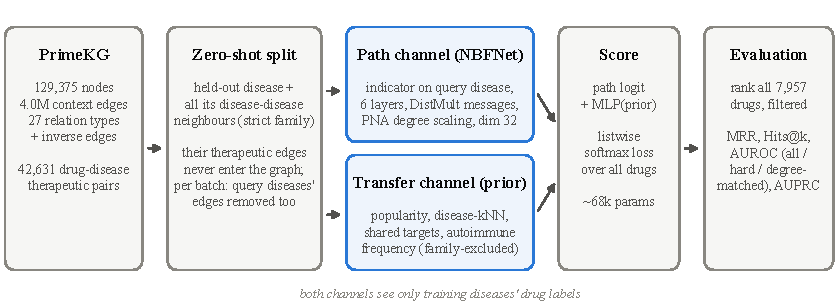
\includegraphics[width=\textwidth]{fig_pipeline.pdf}
\caption{\sysname pipeline. Held-out families never contribute therapeutic edges; both channels see only training diseases' labels; evaluation ranks every drug.}
\label{fig:pipeline}
\end{figure*}

Fig.~\ref{fig:pipeline} gives an overview.

\subsection{Path channel}
For a query $(u, r_q)$, with disease $u$ and query relation ``indication'', NBFNet~\cite{zhu2021nbfnet} computes a representation of every node $v$ that summarises all paths from $u$ to $v$. Node states start from an indicator boundary condition, $h^{(0)}_v=\mathbb{1}[v=u]\,q$, where $q=\mathrm{emb}(r_q)\in\mathbb{R}^{d}$. Each of $L$ layers aggregates relation-specific messages:
\begin{align}
m^{(t)}_v &= \frac{1}{\deg v}\sum_{(x,r,v)\in\mathcal{E}} h^{(t-1)}_x \odot w^{(t)}_{r_q,r} \;+\; \mathbb{1}[v=u]\,q,\label{eq:msg}\\
h^{(t)}_v &= h^{(t-1)}_v + \mathrm{ReLU}\Big(\mathrm{LN}\big(W^{(t)}\big[h^{(t-1)}_v;\, m^{(t)}_v;\, a_v\, m^{(t)}_v\big]\big)\Big).\label{eq:upd}
\end{align}
Here $w^{(t)}_{r_q,r}$ are query-dependent DistMult relation vectors~\cite{yang2015distmult}, $a_v=\log(\deg v+1)/\overline{\log(\deg+1)}$ is a PNA-style degree amplifier~\cite{corso2020pna}, LN is layer normalisation, and the residual connection stabilises the 6-layer network. The path logit of drug $d$ is $s_\text{path}(u,d)=\mathrm{MLP}([h^{(1)}_d;\dots;h^{(L)}_d;q])$. Because propagation starts at $u$, a single forward pass scores all 7,957 drugs. The model needs no trained embedding for $u$, so a disease whose drugs were never seen is handled exactly like any other node.

\subsection{Memory-efficient full-graph propagation}
NBFNet implementations usually materialise per-edge messages, which needs $O(|\mathcal{E}|\,B\,d)$ memory for $B$ queries. That is 4\,M edges $\times$ 8 queries $\times$ 32 dimensions per layer here, and it does not fit on a commodity GPU. We write~\eqref{eq:msg} as $\sum_r (A_r H)\odot w_r$ over 60 sparse CSR adjacency matrices $A_r$. A custom autograd function stores only $H$ and recomputes $A_r H$ in the backward pass, reducing activation memory to $O(|\mathcal{V}|\,B\,d)$. The full graph takes 0.32\,GB. Training with $B=8$ peaks at 5.8\,GB and takes about 8.5\,s per step on an NVIDIA T4, and the gradients pass a finite-difference check.

\subsection{Transfer channel}
The ``++'' component adds four prior features $\phi(u,d)$ per pair:
\begin{enumerate}
\item popularity, the number of training diseases indicated for $d$;
\item a disease-$k$NN transfer score, $\sum_{u'\in\mathcal{N}_k(u)}\mathrm{sim}(u,u')\,y_{u'd}$ with $k=20$ and cosine similarity of TF--IDF-weighted disease--protein and disease--phenotype profiles;
\item the number of $d$'s protein targets associated with $u$;
\item the frequency of $d$ among autoimmune training diseases.
\end{enumerate}
Each feature is computed with $u$'s family excluded, identically in training and testing. A two-layer MLP maps $\phi$ to a logit that is added to the path logit: $s(u,d)=s_\text{path}(u,d)+g(\phi(u,d))$.

\subsection{Objective}
Let $P_u$ be the training indications of $u$. We minimise a multi-positive softmax cross-entropy over all candidates,
\begin{equation}
\mathcal{L}(u)=-\frac{1}{|P_u|}\sum_{d\in P_u}\log\frac{\exp s(u,d)}{\sum_{d'}\exp s(u,d')},
\end{equation}
so every non-indicated drug acts as a negative and no negative sampling is needed. A self-adversarial binary cross-entropy, as used for NBFNet, is evaluated as an ablation.

% =====================================================================
\section{Experimental Setup}
\subsection{Baselines}
All baselines use the same protocol and the same family exclusions.
\emph{Random} ranking.
\emph{Drug degree}: context-graph degree.
\emph{Popularity}: number of training diseases treated.
\emph{Autoimmune frequency}: popularity among autoimmune training diseases.
\emph{Shared targets}: number of the drug's targets associated with the disease.
\emph{Disease $k$NN}: drugs of the 20 most similar training diseases, weighted by similarity.
Disease $k$NN is a transparent version of the ``guilt by association'' rule used throughout repurposing~\cite{bang2023dreamwalk}, and the strongest baseline in our experiments.

\subsection{Metrics}
For disease $u$ with positives $P_u$, each positive $d$ is ranked among all drugs after removing the other positives (filtered rank~\cite{bordes2013transe}). We report
\begin{align}
\mathrm{MRR}_u&=\frac{1}{|P_u|}\sum_{d\in P_u}\frac{1}{\mathrm{rank}_u(d)}, &
\mathrm{H@}k_u&=\frac{1}{|P_u|}\sum_{d\in P_u}\mathbb{1}[\mathrm{rank}_u(d)\le k],
\end{align}
macro-averaged over diseases. MRR originates in question-answering evaluation~\cite{voorhees1999trec} and is the standard KG-completion metric. We also report the share of diseases with at least one positive in the top 10, AUROC and AUPRC over all drugs, AUROC against \emph{hard} negatives (drugs indicated for other autoimmune diseases) and AUROC against \emph{degree-matched} negatives (five drugs of nearest degree per positive). With about 7 positives among 7,957 drugs, random ranking gives MRR $\approx$0.001 and AUPRC $\approx$0.001. AUROC is insensitive to this imbalance~\cite{saito2015prc}, so it is not a headline metric here (Section~\ref{sec:auroc}). For readers outside machine learning we present the metrics in order of interpretability: Any@10 first, then Hits@$k$, AUROC, AUPRC beside its random level, and finally MRR. MRR is easiest to read through ranks: on the test split, \sysname's MRR of \TestMrr{} corresponds to a median known-drug rank of \MedRankTest, with \RankOneShareTest\% of known drugs ranked first. A random ranking puts an approved drug in the top 10 for only \RandExpAnyTenTest\% of test diseases.

\subsection{Statistics}
Models were trained with \MainSeeds{} seeds (0--2) where compute allowed, and one seed for the remaining ablations (stated in each table). Per-disease metrics are first averaged over seeds and then over diseases. We report seed mean $\pm$ sd, percentile bootstrap 95\% CIs over diseases (1,000 resamples)~\cite{efron1993bootstrap}, and, for comparisons, the paired bootstrap CI of the mean difference together with the two-sided Wilcoxon signed-rank test~\cite{wilcoxon1945}. We call a difference significant only if both criteria agree at the 5\% level.

\subsection{Training details}
Hidden size 32, 6 layers, MLP hidden size 64, dropout 0.1, Adam with learning rate $5\times10^{-3}$, batch of 8 query diseases (151 steps per epoch), gradient clipping at 1.0, at most 20 epochs, early stopping on validation MRR with patience 6. The full model has 68,226 parameters. These settings were fixed in advance and were not tuned. Runs used two NVIDIA T4 GPUs (16\,GB each) on Kaggle, were resumable across 12-hour sessions, and stopped early after 10--20 epochs. Transfer runs train on only 11 diseases (2 steps per epoch), so they may run up to 60 epochs with patience 10; all other settings are identical.

% =====================================================================
\section{Results}
\label{sec:results}
We first establish accuracy on unseen diseases (Aim~2), then use the model for the transfer study (Aim~1), and finally analyse its components (Aim~3) and robustness.
\begin{table*}[t]
\centering
\caption{Zero-shot drug ranking over all 7,957 drugs (targets protocol). Models: mean$\pm$sd over seeds ($n$). H@$k$: fraction of a disease's known drugs in the top $k$. AUROC$_\text{hard}$: known drugs vs.\ drugs of other autoimmune diseases.}
\label{tab:main}
\small
\begin{tabular}{lcccccccc}
\toprule
 & \multicolumn{5}{c}{68 zero-shot validation diseases} & \multicolumn{3}{c}{6 rare autoimmune targets}\\
\cmidrule(lr){2-6}\cmidrule(lr){7-9}
Method & MRR & H@1 & H@10 & AUROC & AUROC$_{\text{hard}}$ & MRR & H@10 & AUROC$_{\text{hard}}$\\
\midrule
Random & 0.001 & 0.000 & 0.002 & 0.471 & 0.488 & 0.001 & 0.000 & 0.488\\
Drug degree & 0.004 & 0.000 & 0.003 & 0.783 & 0.421 & 0.003 & 0.000 & 0.404\\
Popularity & 0.046 & 0.034 & 0.049 & 0.830 & 0.476 & 0.099 & 0.148 & 0.460\\
Autoimmune frequency & 0.038 & 0.032 & 0.040 & 0.827 & 0.128 & 0.094 & 0.169 & 0.299\\
Shared targets & 0.057 & 0.032 & 0.105 & 0.845 & 0.530 & 0.008 & 0.000 & 0.491\\
Disease kNN & 0.281 & 0.239 & 0.350 & 0.860 & 0.661 & 0.296 & 0.424 & 0.778\\
\midrule
Prior only (transfer channel) ($n$=1) & 0.303 & 0.265 & 0.353 & 0.884 & 0.707 & 0.322 & 0.483 & 0.782\\
Paths only (NBFNet) ($n$=3) & 0.405$\pm$0.013 & 0.363$\pm$0.019 & 0.479$\pm$0.025 & 0.946$\pm$0.004 & 0.829$\pm$0.011 & 0.463$\pm$0.087 & 0.657$\pm$0.025 & 0.907$\pm$0.007\\
\textbf{BioPathNet++ (paths + prior) ($n$=3)} & 0.394$\pm$0.003 & 0.353$\pm$0.008 & 0.456$\pm$0.018 & 0.938$\pm$0.001 & 0.799$\pm$0.010 & 0.475$\pm$0.017 & 0.648$\pm$0.033 & 0.892$\pm$0.020\\
\bottomrule
\end{tabular}
\end{table*}

\begin{table*}[t]
\centering
\caption{All metrics on the selection-free test split (\TestSeeds{} seed), the validation diseases and the rare targets (seed means). Any@10: diseases with an approved drug in the top 10 (random expectation \RandExpAnyTenTest\%). AUPRC of a random ranking $\approx$ prevalence ($\approx$0.001). Mean rank among 7,957 drugs.}
\label{tab:metrics}
\scriptsize
\setlength{\tabcolsep}{3pt}
\resizebox{\textwidth}{!}{\begin{tabular}{llcccccccccc}
\toprule
Set & Method & Any@10 & H@1 & H@10 & H@50 & AUROC & AUROC$_\text{hard}$ & AUROC$_\text{deg}$ & AUPRC & MRR & Mean rank\\
\midrule
Test (68, never selected) & Random & 1\% & 0.000 & 0.005 & 0.006 & 0.453 & 0.471 & 0.500 & 0.002 & 0.001 & 4,349\\
 & Popularity & 19\% & 0.042 & 0.070 & 0.267 & 0.885 & 0.562 & 0.812 & 0.084 & 0.062 & 918\\
 & Disease $k$NN & 57\% & 0.347 & 0.459 & 0.583 & 0.907 & 0.721 & 0.859 & 0.429 & 0.392 & 742\\
 & \textbf{\sysname} & 76\% & 0.435 & 0.637 & 0.727 & 0.959 & 0.862 & 0.924 & 0.556 & 0.501 & 329\\
\midrule
Validation (68) & Random & 1\% & 0.000 & 0.002 & 0.004 & 0.471 & 0.488 & 0.490 & 0.002 & 0.001 & 4,205\\
 & Popularity & 15\% & 0.034 & 0.049 & 0.188 & 0.830 & 0.476 & 0.760 & 0.069 & 0.046 & 1,355\\
 & Disease $k$NN & 44\% & 0.239 & 0.350 & 0.490 & 0.860 & 0.661 & 0.822 & 0.313 & 0.281 & 1,118\\
 & \textbf{\sysname} & 56\% & 0.353 & 0.456 & 0.601 & 0.938 & 0.799 & 0.886 & 0.424 & 0.394 & 495\\
\midrule
Rare targets (6) & Random & 0\% & 0.000 & 0.000 & 0.000 & 0.476 & 0.488 & 0.389 & 0.002 & 0.001 & 4,165\\
 & Popularity & 50\% & 0.062 & 0.148 & 0.162 & 0.905 & 0.460 & 0.766 & 0.116 & 0.099 & 755\\
 & Disease $k$NN & 67\% & 0.243 & 0.424 & 0.725 & 0.962 & 0.778 & 0.917 & 0.407 & 0.296 & 299\\
 & \textbf{\sysname} & 83\% & 0.396 & 0.648 & 0.695 & 0.982 & 0.892 & 0.954 & 0.594 & 0.475 & 141\\
\bottomrule
\end{tabular}}
\end{table*}

\begin{figure*}[t]
\centering
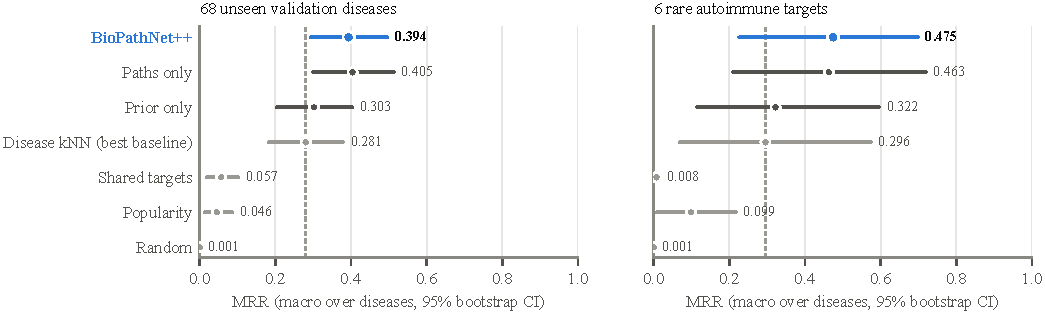
\includegraphics[width=\textwidth]{fig_main_results.pdf}
\caption{MRR with 95\% bootstrap CIs over diseases (seed-averaged). Dashed line: disease $k$NN, the strongest baseline.}
\label{fig:main}
\end{figure*}

\subsection{Aim 2: accuracy on unseen diseases}
\label{sec:aim2}
Table~\ref{tab:metrics} gives every metric for the test split, the validation diseases and the targets. On the test split, never used for training or stopping, an approved drug is in the top 10 for \TabModelTestAnyTen\% of diseases (disease $k$NN \TabKnnTestAnyTen\%, popularity \TabPopTestAnyTen\%, chance \RandExpAnyTenTest\%), and AUPRC is \TabModelTestAuprc{} against a prevalence of about 0.001. Table~\ref{tab:main} and Fig.~\ref{fig:main} compare variants. On the 68 validation diseases, \sysname reaches MRR \MainValidMrr$\pm$\MainValidMrrSd, H@1 \MainValidHitsOne{} and H@10 \MainValidHitsTen. Disease $k$NN reaches \KnnValidMrr, and popularity only \PopValidMrr. The paired MRR gain over disease $k$NN is \DiffMainKnnValid{} (95\% CI \DiffLoMainKnnValid{} to \DiffHiMainKnnValid; Wilcoxon $p$\,\PwilMainKnnValid). The model is better on \WinsMainKnnValid{} diseases, tied on \TiesMainKnnValid{} and worse on \LossesMainKnnValid. The H@10 gain is also significant (\DiffMainKnnValidHitsTen, $p$\,\PwilMainKnnValidHitsTen). For \MainValidAnyTen\% of unseen diseases at least one approved drug appears in the top 10 of 7,957, compared with \KnnValidAnyTen\% for disease $k$NN and \PopValidAnyTen\% for popularity. Against hard negatives (drugs of other autoimmune diseases), AUROC is \MainValidAurocHard, versus \KnnValidAurocHard{} for disease $k$NN and \PopValidAurocHard{} (below chance) for popularity. The model therefore does more than rank generically popular drugs. It outperforms every baseline evaluated on the same leakage-free split. BioPathNet was not run on this split; TxGNN is compared on its own split in Section~\ref{sec:txgnn}.

On the six targets MRR is \MainTargetsMrr$\pm$\MainTargetsMrrSd{} versus \KnnTargetsMrr. The difference (\DiffMainKnnTargets, CI \DiffLoMainKnnTargets{} to \DiffHiMainKnnTargets) points the same way on \WinsMainKnnTargets{} of 6 targets. With six diseases it is not significant (Wilcoxon $p$\,\PwilMainKnnTargets), and we do not claim it is.

\subsubsection{Why AUROC is not the headline metric}
\label{sec:auroc}
Fig.~\ref{fig:auroc} plots AUROC against MRR for every method. Baselines without learning reach AUROC 0.78--0.86, and popularity reaches \PopValidAuroc, yet their MRR is below 0.06. With thousands of negatives per positive, AUROC rewards placing positives above the long tail of irrelevant drugs. It says little about whether a positive reaches the top of the list, which is what a clinician would read. The same effect let a degree heuristic reach AUROC 0.972 in the audit. We therefore headline MRR and Hits@$k$ and report AUROC for completeness (\MainValidAuroc{} validation, \MainTargetsAuroc{} targets).

\begin{figure}[t]
\centering
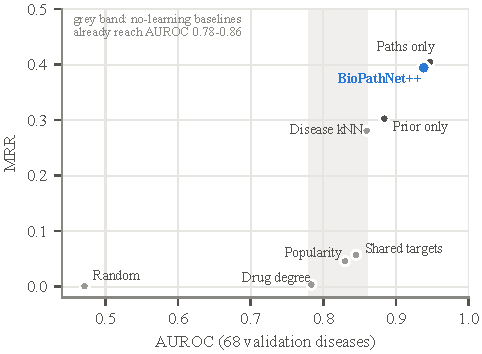
\includegraphics[width=\columnwidth]{fig_auroc_vs_mrr.pdf}
\caption{AUROC vs.\ MRR on the 68 validation diseases. AUROC is high even for no-learning baselines; MRR separates methods.}
\label{fig:auroc}
\end{figure}

\subsection{Aim 1: transfer to rare autoimmune diseases}
\label{sec:aim1}
\begin{figure*}[t]
\centering
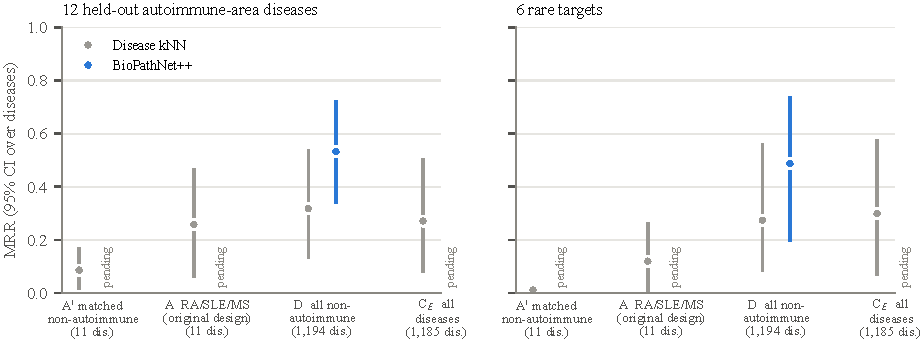
\includegraphics[width=\textwidth]{fig_transfer_curve.pdf}
\caption{Transfer curve (Aim 1). MRR on the 12 held-out autoimmune diseases $E$ (left) and the six rare targets (right) for each training condition, \sysname versus disease $k$NN, with 95\% bootstrap CIs over diseases. A$'$ averages three matched control sets.}
\label{fig:transfer}
\end{figure*}
\begin{table*}[t]
\centering
\caption{Transfer curve: MRR [95\% CI] by training condition. Test diseases are held out in every condition.}
\label{tab:transfercurve}
\small
\begin{tabular}{lrcccc}
\toprule
 & & \multicolumn{2}{c}{12 held-out autoimmune-area diseases (E)} & \multicolumn{2}{c}{6 rare targets}\\
\cmidrule(lr){3-4}\cmidrule(lr){5-6}
Training data & \#dis. & \sysname & disease $k$NN & \sysname & disease $k$NN\\
\midrule
A$'$: 11 matched non-autoimmune diseases & 11 & 0.126 [0.04, 0.22] & 0.086 [0.02, 0.17] & 0.041 [0.00, 0.08] & 0.011 [0.00, 0.02]\\
A: RA/SLE/MS families (11 diseases) & 11 & 0.290 [0.09, 0.50] & 0.258 [0.06, 0.47] & 0.124 [0.01, 0.26] & 0.120 [0.01, 0.26]\\
D: all non-autoimmune diseases & 1,194 & 0.532 [0.34, 0.72] & 0.318 [0.13, 0.53] & 0.487 [0.20, 0.73] & 0.273 [0.08, 0.56]\\
C$_E$: all diseases except the test set & 1,185 & 0.452 [0.25, 0.67] & 0.271 [0.08, 0.50] & 0.550 [0.28, 0.78] & 0.299 [0.07, 0.57]\\
\bottomrule
\end{tabular}
\end{table*}
Fig.~\ref{fig:transfer} and Table~\ref{tab:transfercurve} give the transfer curve.
\emph{Scarce data.} Trained only on the RA/SLE/MS families (A), \sysname reaches MRR \TrAEMrr{} on $E$, against \TrActlEMrr{} when trained on label-matched non-autoimmune diseases (A$'$). The paired difference of \DiffTrAActlE{} (CI \DiffLoTrAActlE{} to \DiffHiTrAActlE; Wilcoxon $p$\,\PwilTrAActlE; better on \WinsTrAActlE{} of 12 diseases) is significant. It also holds when each run's final checkpoint is used instead of the early-stopped one (\DiffTrAActlELast, CI \DiffLoTrAActlELast{} to \DiffHiTrAActlELast, $p$\,\PwilTrAActlELast). The rare targets point the same way (\TrATargetsMrr{} vs.\ \TrActlTargetsMrr; $p$\,\PwilTrAActlTargets, $n=6$). The disease-$k$NN baseline shows the same pattern (\TrAEKnnMrr{} vs.\ \TrActlEKnnMrr), and in this regime the model is only slightly ahead of it. With 11 training diseases, the transferable knowledge is essentially a drug-class prior. The RA/SLE/MS families are treated mostly with corticosteroids and TNF inhibitors, and the A-trained model ranks the same corticosteroids first for every target. That is a reasonable first guess for an autoimmune disease, but it is not disease-specific reasoning. To test whether path reasoning itself transfers in this regime, rather than only the drug-class prior carried by the transfer channel, we repeated A and A$'$ with paths only: \TrAPathsEMrr{} vs.\ \TrActlPathsEMrr{} (difference \DiffTrAActlPathsE, CI \DiffLoTrAActlPathsE{} to \DiffHiTrAActlPathsE; $p$\,\PwilTrAActlPathsE).
% RECHECK after Kaggle session 5: interpret the paths-only A vs A' result in the sentence above.

\emph{Full scale.} Broad training data without any autoimmune disease (D) raises accuracy on $E$ to \TrDEMrr. Adding the autoimmune diseases (C$_E$, one seed) gives \TrCEEMrr{} (difference \DiffTrCEDE, $p$\,\PwilTrCEDE), with no measurable gain. On the rare targets, removing all autoimmune diseases likewise leaves MRR unchanged (\NoautoTargetsMrr{} vs.\ \MainTargetsMrr; \NoautoSeeds{} seeds each; $p$\,\PwilMainNoautoTargets).
Aim~1 is therefore answered in two parts. The model's zero-shot transfer works at every scale we tested (Aim~2). Its best \emph{source} depends on how much data is available: related autoimmune diseases when training data is scarce, and the broad pharmacological graph, which then makes autoimmune data unnecessary, at full scale.
One caveat concerns model selection. The A and A$'$ runs early-stop on the 68 general validation diseases, on which all of them score MRR below 0.05, so the selected epoch can be very early (epoch 0 for one A seed). Training on 11 diseases is also unstable: one A seed falls from 0.29 to 0.09 MRR on $E$ by its final epoch. The final-checkpoint analysis above shows that the A versus A$'$ conclusion does not depend on this choice.

\subsubsection{Transfer at full scale}
\begin{table}[t]
\centering
\caption{Effect of removing all 123 autoimmune diseases from training.}
\label{tab:transfer}
\small
\setlength{\tabcolsep}{3pt}
\resizebox{\columnwidth}{!}{\begin{tabular}{lcccc}
\toprule
Training data & \multicolumn{2}{c}{6 targets} & \multicolumn{2}{c}{21 autoimmune-area diseases}\\
\cmidrule(lr){2-3}\cmidrule(lr){4-5}
 & MRR & H@10 & MRR & H@10\\
\midrule
BioPathNet++, all diseases in training ($n$=3) & 0.475$\pm$0.017 & 0.648$\pm$0.033 & -- & --\\
BioPathNet++, 123 autoimmune diseases removed ($n$=1) & 0.473 & 0.628 & 0.485 & 0.608\\
Paths only, 123 autoimmune diseases removed & \multicolumn{4}{c}{pending}\\
Disease kNN (no-autoimmune pool) & 0.273 & 0.594 & 0.311 & 0.469\\
\bottomrule
\end{tabular}}
\end{table}
Table~\ref{tab:transfer} repeats the question at full scale on all 21 area diseases. With all 123 autoimmune nodes removed from training, target MRR is \NoautoTargetsMrr$\pm$\NoautoTargetsMrrSd{} versus \MainTargetsMrr$\pm$\MainTargetsMrrSd{} with them (\NoautoSeeds{} seeds each; paired difference with minus without \DiffMainNoautoTargets{}, CI \DiffLoMainNoautoTargets{} to \DiffHiMainNoautoTargets, $p$\,\PwilMainNoautoTargets). Removing autoimmune training data does not hurt the autoimmune targets. On the 21 held-out autoimmune-area diseases, which are never used for selection, the model reaches MRR \NoautoAreaMrr$\pm$\NoautoAreaMrrSd{} versus \NoautoKnnAreaMrr{} for disease $k$NN. The difference is \DiffNoautoKnnArea{} (CI \DiffLoNoautoKnnArea{} to \DiffHiNoautoKnnArea), but the Wilcoxon test gives $p$\,\PwilNoautoKnnArea, so by our criterion it is suggestive rather than significant. The autoimmune-specific transfer hypothesis is therefore not supported. Whatever transfers comes from the general pharmacology and biology encoded in the KG, not from autoimmune training labels.

In this harder setting the transfer channel may help. On the area diseases, paths only (one seed) reaches \NoautoPathsAreaMrr{} against the full model's \NoautoAreaMrr{} (difference \DiffNoautoPathsArea, CI \DiffLoNoautoPathsArea{} to \DiffHiNoautoPathsArea, $p$\,\PwilNoautoPathsArea). This is not significant, and more paths-only seeds are needed before claiming it.

\subsection{Aim 3: what each component contributes}
\label{sec:aim3}
\begin{table}[t]
\centering
\caption{Ablations (targets protocol). $p$: two-sided Wilcoxon on paired validation MRR vs.\ the full model.}
\label{tab:ablation}
\small
\setlength{\tabcolsep}{3pt}
\resizebox{\columnwidth}{!}{\begin{tabular}{lcccc}
\toprule
Variant (seed 0 unless noted) & Valid MRR & Valid H@10 & Targets MRR & $p$ vs full (valid)\\
\midrule
Full model ($n$=3) & 0.394$\pm$0.003 & 0.456$\pm$0.018 & 0.475$\pm$0.017 & --\\
$-$ transfer channel ($n$=3) & 0.405$\pm$0.013 & 0.479$\pm$0.025 & 0.463$\pm$0.087 & 0.148\\
$-$ path reasoning (prior only) & 0.303 & 0.353 & 0.322 & $<$0.001\\
BRG relation subset & 0.397 & 0.488 & 0.424 & 0.906\\
BCE loss instead of listwise & 0.347 & 0.434 & 0.292 & 0.005\\
\bottomrule
\end{tabular}}
\end{table}
Table~\ref{tab:ablation} isolates the components. Without the transfer channel (paths only), validation MRR is \PathsValidMrr{}, statistically tied with the full model (difference \DiffMainPathsValid, $p$\,\PwilMainPathsValid). Without path reasoning (transfer channel only), MRR falls to \PriorValidMrr{} ($p$\,\PwilMainPriorValid), close to disease $k$NN, which is one of its inputs. Path reasoning is therefore the source of the gain. The transfer channel does not change the mean. It does reduce variability across seeds on the targets, from sd \PathsTargetsMrrSd{} to \MainTargetsMrrSd{} (Fig.~\ref{fig:pertarget}), which matters in practice because a ranking used for case studies should not depend on the seed. An earlier interim claim that the channel improved rare-target accuracy, based on one seed, did not survive replication and was withdrawn.

Two further single-seed ablations change one design choice each.
\emph{Loss.} Replacing the listwise softmax with NBFNet's self-adversarial BCE lowers validation MRR to \BceValidMrr{}. Against the seed-averaged full model the gap is \DiffMainBceValid{} (Wilcoxon $p$\,\PwilMainBceValid). Against the same seed alone it is \DiffSzeroMainBceValid{} (CI \DiffLoSzeroMainBceValid{} to \DiffHiSzeroMainBceValid; $p$\,\PwilSzeroMainBceValid), so the advantage is consistent but borderline for one seed. Scoring all drugs in the loss matches how the model is evaluated, which is a plausible reason for the gain.
\emph{Background graph.} Following BioPathNet's background regulatory graph~\cite{hu2026biopathnet}, we drop the two largest and least mechanistic relation families: tissue expression and drug--drug interactions. This shrinks the context graph from \EdgesMain{} to \EdgesBrg{} edges (\BrgEdgeCutPct\% fewer). Validation MRR is unchanged (\BrgValidMrr; $p$\,\PwilMainBrgValid), and steps are \BrgSpeedupPct\% faster (\StepSecBrg{} vs.\ \StepSecMain\,s) with lower peak memory (\PeakMemBrg{} vs.\ \PeakMemMain\,GB). Most of PrimeKG's edges are therefore redundant for this task, in line with BioPathNet's relation ablation~\cite{hu2026biopathnet}, and a 3.5$\times$ smaller graph is a practical option for limited hardware.

\subsection{Robustness: sparsity, selection bias and a selection-free test}
\label{sec:robust}
Validation diseases also select the stopping epoch, so validation scores are optimistic. From the training logs, the gap between the best-epoch and last-epoch validation MRR is \SelGapMainMin--\SelGapMainMax{} for the full model and \SelGapPathsMin--\SelGapPathsMax{} for paths only. This is an order of magnitude smaller than the gain over disease $k$NN (\DiffMainKnnValid), but larger than the difference between the full model and paths only, so the latter is a tie. The targets and the 21 area diseases are untouched by selection, and their results agree with the validation conclusions.


\subsubsection{Selection-free test split}
\begin{table}[t]
\centering
\caption{Selection-free test split: 68 diseases never used for training or early stopping.}
\label{tab:test}
\small
\setlength{\tabcolsep}{3pt}
\resizebox{\columnwidth}{!}{\begin{tabular}{lccc}
\toprule
Method (68 test diseases, never used for training or stopping) & MRR & H@10 & AUROC$_\text{hard}$\\
\midrule
Random & 0.001 & 0.005 & 0.471\\
Popularity & 0.062 & 0.070 & 0.562\\
Disease $k$NN & 0.392 & 0.459 & 0.721\\
\textbf{\sysname} & \multicolumn{3}{c}{pending}\\
\bottomrule
\end{tabular}}
\end{table}
On the selection-free test split (Table~\ref{tab:test}), \sysname reaches MRR \TestMrr{} and H@10 \TestHitsTen, against \KnnTestMrr{} and \KnnTestHitsTen{} for disease $k$NN (paired difference \DiffTestKnn, CI \DiffLoTestKnn{} to \DiffHiTestKnn, $p$\,\PwilTestKnn; \TestSeeds{} seed, with two more seeds resuming). For \TestAnyTen\% of the test diseases an approved drug appears in the top 10 (disease $k$NN: \KnnTestAnyTen\%). The same model reaches \TestModelValidMrr{} on its validation diseases. Test diseases are drawn from non-autoimmune diseases and are easier for every method (disease $k$NN also rises from \KnnValidMrr{} to \KnnTestMrr), so the two levels are not directly comparable. What matters is that the gain over the baseline holds on diseases that no model choice has seen.

\subsubsection{Head-to-head with TxGNN on its own split}
\label{sec:txgnn}
\begin{table}[t]
\centering
\caption{TxGNN's autoimmune disease-area split, generated by TxGNN's own code; both models trained on the same graph, one seed each. TxGNN protocol: drugs with at least one indication are ranked; full ranking: all drugs. The published row is from TxGNN's repository (different random draw of the split).}
\label{tab:txgnn}
\small
\setlength{\tabcolsep}{3pt}
\resizebox{\columnwidth}{!}{\begin{tabular}{lccccccc}
\toprule
 & & \multicolumn{3}{c}{TxGNN protocol} & \multicolumn{3}{c}{full ranking}\\
\cmidrule(lr){3-5}\cmidrule(lr){6-8}
Method & seeds & R@100 & AUROC & AUPRC & MRR & H@100 & AUROC\\
\midrule
TxGNN, published & 5 & 0.338 & -- & -- & -- & -- & --\\
\midrule
\multicolumn{8}{l}{\emph{Full training coverage (main comparison)}}\\
TxGNN & 3 & 0.536 & 0.901 & 0.161 & 0.048 & 0.232 & 0.753\\
\sysname (1,139 train dis.) & 3 & 0.614 & 0.777 & 0.343 & 0.273 & 0.618 & 0.936\\
\midrule
\multicolumn{8}{l}{\emph{Strict coverage: every disease with a test edge held out (ablation)}}\\
TxGNN (unchanged) & 1 & 0.474 & 0.909 & 0.147 & 0.026 & 0.155 & 0.736\\
\sysname (637 train dis.) & 1 & 0.475 & 0.746 & 0.101 & 0.061 & 0.398 & 0.910\\
\bottomrule
\end{tabular}}
\end{table}
For a direct comparison we ran both models on TxGNN's own autoimmune disease-area split, generated by TxGNN's code (commit \texttt{0e0203c}). Its random test edges are drawn without a seed, so we fixed the seed; this draw therefore differs from the published runs. We converted the split to our format so that both models see the same training graph. The test set is the \TxhN{} held-out area diseases that have indications (\TxhPairs{} drug--disease pairs). TxGNN was trained with the settings of its reproduction script: one full pre-training epoch (\TxhPretrainH{}~h on a T4) and 500 fine-tuning epochs; its validation AUROC was still rising slightly in the last epochs. To keep every TxGNN test edge out of our message graph, the conversion also holds out every disease with any test edge, together with its family. \sysname therefore trained on \TxhTrainDis{} diseases (plus \TxhValidDis{} for early stopping), whereas TxGNN learns from the training edges of all \TxhNonTestDis{} non-test diseases; this handicap works against our model. As a check of the evaluation code, our implementation of TxGNN's protocol reproduces TxGNN's own evaluation of its predictions exactly (Recall@100 \TxhTxOfficialRecall{}, higher than the published \TxhTxPublishedRecall{} for a different draw of the split).

The two protocols disagree (Table~\ref{tab:txgnn}). TxGNN's protocol ranks only the \TxhCand{} drugs that have at least one indication. There, Recall@100 is tied (\TxhOursRecall{} for \sysname, \TxhTxRecall{} for TxGNN; difference \TxhDiffRecall, CI \TxhDiffLoRecall{} to \TxhDiffHiRecall, $p$\,\TxhPwilRecall), and TxGNN separates the true drugs better by AUROC (\TxhTxAuroc{} against \TxhOursAuroc; difference \TxhDiffAuroc, CI \TxhDiffLoAuroc{} to \TxhDiffHiAuroc, $p$\,\TxhPwilAuroc; TxGNN better on \TxhLossesAuroc{} of \TxhN{} diseases). AUPRC does not differ significantly (\TxhDiffAuprc, $p$\,\TxhPwilAuprc). When all 7,957 drugs are ranked, the order reverses. \sysname has higher H@100 (\TxhOursHitsHund{} against \TxhTxHitsHund; difference \TxhDiffFullHitsHund, CI \TxhDiffLoFullHitsHund{} to \TxhDiffHiFullHitsHund, $p$\,\TxhPwilFullHitsHund) and higher AUROC (\TxhOursFullAuroc{} against \TxhTxFullAuroc; \TxhDiffFullAuroc, CI \TxhDiffLoFullAuroc{} to \TxhDiffHiFullAuroc, $p$\,\TxhPwilFullAuroc). Its MRR is higher on \TxhWinsFullMrr{} of \TxhN{} diseases (\TxhOursMrr{} against \TxhTxMrr, $p$\,\TxhPwilFullMrr), but the confidence interval includes zero (\TxhDiffLoFullMrr{} to \TxhDiffHiFullMrr), so by our rule this difference is not significant. The ranked lists explain the reversal: only \TxhTxIndShare\% of TxGNN's top-100 drugs have an indication for any disease in the graph, against \TxhOursIndShare\% for \sysname. TxGNN places many drugs without any indication in the graph near the top, and its protocol removes them before scoring; \sysname ranks such drugs low but separates the true drugs from other indicated drugs less sharply. Neither model dominates. With one seed per model and \TxhN{} test diseases, this comparison is a first data point, not a ranking of the two methods.

\subsubsection{Sparsity}
\begin{figure}[t]
\centering
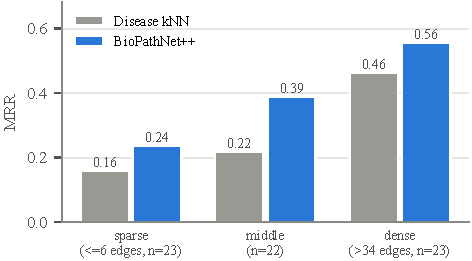
\includegraphics[width=\columnwidth]{fig_sparsity.pdf}
\caption{Validation MRR by connectivity tertile of the held-out disease (number of context edges).}
\label{fig:sparsity}
\end{figure}
Rare diseases are sparsely annotated, so we stratify the validation diseases by their number of context edges (Fig.~\ref{fig:sparsity}). Accuracy grows with connectivity (Spearman $\rho=\RhoMain$, $p$\,\RhoPMain). \sysname is ahead of disease $k$NN in every tertile: \TertMainLow{} vs.\ \TertKnnLow{} for the sparsest third, \TertMainMid{} vs.\ \TertKnnMid{} in the middle, and \TertMainHigh{} vs.\ \TertKnnHigh{} for the densest third. The relative gain is largest in the middle tertile. Diseases with almost no molecular annotation remain the hardest case for every method.

\subsection{Case studies}
\begin{table}[t]
\centering
\caption{Per-target MRR (seed mean) and the model's top predictions (seed 0). $^{*}$\,labelled in PrimeKG.}
\label{tab:targets}
\scriptsize
\setlength{\tabcolsep}{2.5pt}
\resizebox{\columnwidth}{!}{\begin{tabular}{lcccccl}
\toprule
Target & \#known & kNN & Paths only & BioPathNet++ & Best rank & Top-3 predictions (seed 0)\\
\midrule
PBC & 1 & 1.000 & 1.000 & 1.000 & 1 & Ursodeoxycholic acid$^{*}$, Doripenem, Cholic Acid\\
SSc & 5 & 0.041 & 0.437 & 0.452 & 1 & Benzoic acid$^{*}$, Bosentan$^{*}$, Limaprost\\
Sj\"ogren & 12 & 0.152 & 0.731 & 0.510 & 1 & Prednisolone$^{*}$, Polyethylene glycol 400$^{*}$, Propylene glycol$^{*}$\\
AIH & 1 & 0.001 & 0.002 & 0.002 & $>$100 & Prednisolone, Triamcinolone, Hydrocortisone\\
MG & 7 & 0.179 & 0.418 & 0.671 & 1 & Ambenonium$^{*}$, Neostigmine$^{*}$, Pyridostigmine$^{*}$\\
Crohn & 24 & 0.403 & 0.191 & 0.212 & 1 & Hydrocortisone$^{*}$, Triamcinolone$^{*}$, Cortisone acetate$^{*}$\\
\bottomrule
\end{tabular}}
\end{table}
\begin{figure}[t]
\centering
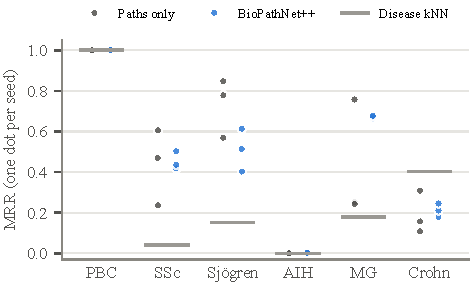
\includegraphics[width=\columnwidth]{fig_per_target.pdf}
\caption{Per-target MRR for each seed. The transfer channel narrows the spread across seeds (SSc, Sj\"ogren, MG).}
\label{fig:pertarget}
\end{figure}
Table~\ref{tab:targets} and Fig.~\ref{fig:pertarget} show the six targets.
\textbf{PBC.} Ursodeoxycholic acid, the first-line therapy and the only labelled drug, is ranked first in all seeds. Cholic acid and dehydrocholic acid, which are also bile acids, follow.
\textbf{MG.} The four labelled cholinesterase inhibitors (ambenonium, neostigmine, pyridostigmine, distigmine) are ranked 1--4 in all seeds.
\textbf{SSc.} The labelled drugs aminobenzoic acid, benzoic acid and bosentan lead, followed by corticosteroids.
\textbf{Sj\"ogren.} Labelled tear-substitute components (propylene glycol, povidone, polysorbate~80) and prednisolone lead.
\textbf{Crohn.} Labelled corticosteroids hold ranks 1--4. Mesalazine (off-label) and fluoroquinolones follow, but many of the 24 labelled drugs rank low, which keeps MRR modest.
\textbf{AIH.} The model fails by the metric but arguably not clinically. PrimeKG lists a single off-label drug for AIH, while the model ranks prednisolone first in two of three seeds. Corticosteroids are standard AIH therapy and the comparator arm in AIH trials (prednisone in NCT00838214). This is a label gap, and it shows that metric values on sparsely labelled diseases are lower bounds.

\subsection{Validation of the predictions}
\label{sec:validation}
Ranking metrics only reward drugs that PrimeKG already labels. To judge the model's \emph{unlabelled} candidates, we built five further validation layers (\texttt{bpp/validate.py}; every API response is cached with the code). The candidate set is each target's top 20 by rank averaged over the three seeds; \ValNovelN{} of these 120 are unlabelled. We compare them with two reference sets: the popularity baseline's top 20 unlabelled drugs and 20 random unlabelled drugs per target (Table~\ref{tab:validation}).

\begin{table}[t]
\centering
\caption{Evidence for unlabelled candidates: \sysname{} top-20 vs.\ popularity top-20 vs.\ random drugs (six targets).}
\label{tab:validation}
\scriptsize
\setlength{\tabcolsep}{2.5pt}
\resizebox{\columnwidth}{!}{\begin{tabular}{lccc}
\toprule
Evidence for unlabelled candidates & \sysname{} top-20 ($n$=86) & Popularity top-20 ($n$=120) & Random ($n$=120)\\
\midrule
Trial evidence, grade A--C (ClinicalTrials.gov) & 19\% & 15\% & 1\%\\
Trial evidence, phase $\geq$2 (grade A--B) & 16\% & 13\% & 0\%\\
Any PubMed co-mention & 63\% & 72\% & 18\%\\
PubMed title supports use & 24\% & 16\% & 0\%\\
PubMed title reports harm / no benefit & 4\% & 12\% & 0\%\\
$\geq$1 drug target among disease genes & 17\% & 16\% & 3\%\\
\bottomrule
\end{tabular}}
\end{table}

\textbf{Clinical trials.} We searched ClinicalTrials.gov (API v2) for each drug and disease, with disease synonyms. A trial counts only if it names the drug as an intervention, and we record whether the drug is in an experimental or comparator arm. Grades: A, phase $\geq$3; B, phase 2; C, phase 1 or observational; D, none. \ValTrialModel\% of the model's unlabelled candidates have such a trial (\ValGradeA{} at phase $\geq$3), against \ValTrialPop\% for popularity and \ValTrialRand\% for random drugs. Examples are amifampridine for MG (NCT03304054), ciprofloxacin and clarithromycin for Crohn, and ustekinumab for Crohn, which the FDA approved for Crohn in 2016 but PrimeKG does not label. Some grades for PBC and AIH come from PBC--AIH overlap-syndrome trials.

The same check on the C$_E$ transfer model's top 10 for the 12 held-out autoimmune-area diseases finds an approved drug in the top 10 for \EcheckDiseases{} of 12 diseases. \EcheckNovelTrial{} of its \EcheckNovel{} unlabelled top-10 drugs have a registered trial for the disease, among them canakinumab for CINCA syndrome, which has phase~3 trials (NCT00685373) (\texttt{transfer\_E\_top10.csv}).

\textbf{Literature.} For each pair we retrieved the PubMed hit count for ``drug''[tiab] AND ``disease''[tiab] and the three most relevant titles. The titles were classified as supporting, mixed, against or unrelated with AI assistance; the authors still need to verify these labels (\texttt{literature\_labels.csv}). The model's candidates are co-mentioned with their disease somewhat less often than popular drugs (\ValLitHitModel\% vs.\ \ValLitHitPop\%), but more often in supporting titles (\ValLitSupModel\% vs.\ \ValLitSupPop\%; random \ValLitSupRand\%). They are also rarely in titles that report harm (\ValLitAgainstModel\% vs.\ \ValLitAgainstPop\%). The model's harmful pairs are corticosteroids in SSc, where high doses are linked to scleroderma renal crisis; popularity's are mostly antibiotics that can worsen MG or induce autoimmune hepatitis.

\textbf{Temporal validation.} PrimeKG's drug labels predate 2022. Of the drugs approved for our targets since then, six are drug nodes in PrimeKG (Table~\ref{tab:temporal}); seladelpar, efgartigimod, zilucoplan, nipocalimab and mirikizumab are absent. Their median rank is \TempPostMedRank{} of 7,957 (top \TempPostMedPct\%), and \TempPostBetter{} of 6 rank better than the random median. Risankizumab, the first IL-23 inhibitor approved for Crohn (2022), ranks \TempRankRisankizumab. Elafibranor, a PPAR agonist for PBC, ranks in the bottom third. With six drugs the trend is not significant (sign test $p$\,\TempPostP), and disease $k$NN ranks three of the six higher. Three older approvals that PrimeKG fails to label are reported separately: obeticholic acid, nintedanib and tocilizumab. Tocilizumab for SSc-associated lung disease ranks \TempRankTocilizumab.

\begin{table}[t]
\centering
\caption{Ranks of drugs approved for a target after the PrimeKG snapshot (top block) and of earlier approvals missing from PrimeKG's labels (bottom). Mean rank over three seeds; dates from the manufacturers' or FDA announcements.}
\label{tab:temporal}
\scriptsize
\setlength{\tabcolsep}{2.5pt}
\resizebox{\columnwidth}{!}{\begin{tabular}{llccccc}
\toprule
Drug & Target & FDA approval & \sysname{} rank & Top \% & $k$NN rank & Popularity rank\\
\midrule
Risankizumab & Crohn & 2022-06 & 37 & 0.5 & 30 & 951\\
Upadacitinib & Crohn & 2023-05 & 550 & 6.9 & 127 & 1,527\\
Ravulizumab & MG & 2022-04 & 845 & 10.6 & 1,383 & 1,381\\
Guselkumab & Crohn & 2025-03 & 1,363 & 17.1 & 5,570 & 5,570\\
Rozanolixizumab & MG & 2023-06 & 2,278 & 28.6 & 7,182 & 7,182\\
Elafibranor & PBC & 2024-06 & 5,825 & 73.2 & 3,266 & 3,266\\
\midrule
Tocilizumab & SSc & 2021-03 & 58 & 0.7 & 35 & 260\\
Nintedanib & SSc & 2019-09 & 848 & 10.7 & 375 & 365\\
Obeticholic acid & PBC & 2016-05 & 2,272 & 28.6 & 6,452 & 6,452\\
\bottomrule
\end{tabular}}
\end{table}

\textbf{Mechanism.} Using PrimeKG's drug--target and disease--gene edges, \ValDisGeneModel\% of the model's unlabelled candidates have at least one target among the disease's genes, against \ValDisGenePop\% for popularity and \ValDisGeneRand\% for random drugs. A hypergeometric test for enrichment of drug targets in 109 immune-related Reactome pathways (Benjamini--Hochberg corrected) found no significant enrichment in any set. Most candidates have few annotated targets, so this test has little power.

\textbf{Path explanations.} We extract the paths behind a prediction by gradient-times-input attribution on every edge's message, followed by beam search over the most important edges~\cite{zhu2021nbfnet} (\texttt{bpp/explain.py}). A check confirms that the attribution pass reproduces the model's scores exactly. Table~\ref{tab:paths} shows four examples. The cholinesterase inhibitors reach MG through the MuSK gene and neuromuscular-junction disease, and amifampridine through its indication for Lambert--Eaton myasthenic syndrome. Ursodeoxycholic acid reaches PBC through biliary-tract diseases. The paths also expose weak predictions: ciprofloxacin reaches Crohn through ``mouth disease'' and sinusitis, not through its documented use in perianal disease.

\begin{table*}[t]
\centering
\caption{Highest-scoring explanation path for four predictions (main model, seed 0); edge labels are PrimeKG relations ($^{-1}$: inverse direction).}
\label{tab:paths}
\scriptsize
\begin{tabular}{p{0.97\linewidth}}
\toprule
\textbf{Pyridostigmine for Myasthenia Gravis}: myasthenia gravis $\xrightarrow{\text{disease protein$^{-1}$}}$ MUSK $\xrightarrow{\text{disease protein}}$ neuromuscular junction disease $\xrightarrow{\text{indication (disease$\to$drug)}}$ Pyridostigmine\\[2pt]
\textbf{Ursodeoxycholic acid for Primary Biliary Cholangitis}: primary biliary cholangitis $\xrightarrow{\text{disease disease}}$ genetic biliary tract disease $\xrightarrow{\text{disease disease}}$ choledocholithiasis $\xrightarrow{\text{indication (disease$\to$drug)}}$ Ursodeoxycholic acid\\[2pt]
\textbf{Amifampridine for Myasthenia Gravis}: myasthenia gravis $\xrightarrow{\text{disease disease}}$ immune-mediated acquired neuromuscular junction disease $\xrightarrow{\text{disease disease$^{-1}$}}$ Lambert-Eaton myasthenic syndrome $\xrightarrow{\text{indication (disease$\to$drug)}}$ Amifampridine\\[2pt]
\textbf{Ciprofloxacin for Crohn Disease}: Crohn disease $\xrightarrow{\text{disease disease$^{-1}$}}$ mouth disease $\xrightarrow{\text{disease disease}}$ maxillary sinusitis $\xrightarrow{\text{indication (disease$\to$drug)}}$ Ciprofloxacin\\[2pt]
\bottomrule
\end{tabular}
\end{table*}

\textbf{Drug classes and popularity bias.} By name, corticosteroids fill \ValSteroidShare\% and antibacterials \ValAntibioticShare\% of all 120 top-20 slots. DRKG's DrugBank-to-ATC links cover only \ValAtcCoverage\% of the candidates, so we use the drug names as the primary class signal and report ATC codes alongside. As an exploratory complement we re-rank each target after regressing out log popularity. The resulting ``less obvious'' lists include amifampridine and guanidine for MG, lifitegrast for Sj\"ogren and the IL-23 inhibitor tildrakizumab for Crohn (\texttt{popularity\_adjusted\_candidates.csv}).

\textbf{Expert review.} The top 10 per target, with all evidence columns and an empty 1--5 plausibility column, are prepared for clinical review (\texttt{expert\_review\_sheet.xlsx}).

% =====================================================================
\section{Discussion}
\label{sec:discussion}
\subsection{How good are these numbers?}
Two comparisons matter. Against chance and simple rules, the model improves MRR from 0.001 (random) and \PopValidMrr{} (popularity) to \MainValidMrr{}, and it is significantly better than a strong, interpretable similarity baseline. Against the literature, BioPathNet reports zero-shot indication MRR from about 0.2 to above 0.6 across disease areas, and Hits@10 from 30\% to 100\%~\cite{hu2026biopathnet}. Our values fall inside that range. The protocols differ, however. BioPathNet and TxGNN hold out disease areas and remove 95\% of their molecular edges, whereas we hold out families and keep molecular context. TxGNN's AUPRC uses one sampled negative per positive, while our AUPRC uses all drugs. We therefore do not compare with their reported numbers, and compare with TxGNN only on a shared split (its own; Section~\ref{sec:txgnn}). BioPathNet has not yet been run on a shared split.

\subsection{Why the earlier numbers looked better}
The earlier pipeline reported AUPRC up to 0.999 because it measured a different and easier quantity: separating known pairs, which were already in the graph, from random pairs. Values near 0.99 are common in medical classification tasks, where each decision has two classes. In ranking thousands of drugs for an unseen disease, the field's best reported MRRs lie well below 1. Reviewers should be sceptical of near-perfect zero-shot numbers.

\subsection{Limitations}
(i) The targets have 1--24 labelled drugs, and PBC and AIH have one each, so per-target metrics are noisy and can be lower bounds (AIH).
(ii) Validation diseases select the epoch; the selection-free test split (Section~\ref{sec:robust}) bounds this bias. (iii) TxGNN's autoimmune area also contains autoinflammatory and non-specific nodes (e.g.\ familial Mediterranean fever, ``autoimmune disease''), and the transfer test set $E$ has only 12 diseases.
(iv) Some ablations use one seed.
(v) The model favours corticosteroids and antibiotics across immune diseases (\ValSteroidShare\% and \ValAntibioticShare\% of top-20 slots). This is clinically sensible for corticosteroids but partly popularity bias.
(vi) PrimeKG labels are incomplete and partly derived from curated resources, so true repurposing candidates are scored as false positives.
(vii) The test split has \TestSeeds{} seed so far. Literature titles were classified with AI assistance and are pending author verification. The temporal test covers only six drugs.
(viii) No clinician has reviewed the candidates yet. The rankings are hypotheses for research, not treatment recommendations.

% =====================================================================
\section{Conclusion}
Path-based zero-shot transfer works for rare autoimmune diseases that a model has never seen. The best source of the transferred knowledge depends on how much data is available. With only a handful of training diseases, related autoimmune diseases provide the most useful signal. With the full knowledge graph, autoimmune training data adds nothing measurable, and accuracy comes from broad pharmacological and biological structure. On a strict-family protocol with full ranking over all drugs, the path-based \sysname outperforms every baseline evaluated on the same split. It recovers established therapies for several rare autoimmune diseases on a single commodity GPU. Path reasoning drives accuracy, the transfer channel adds stability, and most of the graph's edges are redundant. An audit of an earlier pipeline shows how leakage and random negatives can produce near-perfect but meaningless scores. Its unlabelled candidates are enriched for registered trials, and it ranks drugs approved after its training data above chance. Future work: more seeds of the TxGNN comparison, BioPathNet and KG-embedding baselines on a shared split, a three-seed test split, and clinician review of the candidates using the prepared review sheet.

\section*{Data and Code Availability}
PrimeKG is available from Harvard Dataverse (doi:10.7910/DVN/IXA7BM). Code, splits, the audit script, run logs and the analysis that generates every number and table in this paper are in the project repository.

\section*{Acknowledgment}
The authors thank their guide, Dr.\ Priyanka H., PES University, for supervising this work.
% IEEE policy requires disclosure of AI-generated content; edit to describe actual use.
Generative AI tools were used to assist with code development, data analysis and language editing. All results were verified by the authors against the released run logs.

\bibliographystyle{IEEEtran}
\bibliography{references}

\end{document}
